\section{Instrumentation}

There are two main challenges on tracing processes' progress with binary instrumentation approaches in production systems. One is the performance issue. Even a lightweight static binary instrumentation usually pulls down execution time in several to several tens percentage, leading to speculative executions pyrrhic.  The other one is about exactness accuracy. The ideal progress tracing is uniform with the real execution, which means that it can estimate accurately how much the task has been done and how long it will still last? Taking downloading a file for example, if the downloading progress bar shows a 50\% completion after 1 minute, it is clear about that half of the task has been done and it may still last about another 1 minute with a not too bad network. But for a compute-intensive process, we can only know the process has met which tracepoint we instrumented. We can never know the actions of the process that have no instrumented tracepoint, and the same to the subsequent actions of the process. So the progress of a compute-intensive process not related to the input/output (I/O) is hard to estimate.

We primarily concern about the performance of tracing in NO2's instrumentation, and then overcome the second dilemma with NO2's outliers clustering requiring no accurate estimate of progress, discussed in the next section.

With lots of case study, we refine two simple rules of binaries' runtime behaviors. Functions in a binary code can be placed in different level of an abstract syntax tree (AST). Functions in same level are often called with frequencies at similar order of magnitude in a range of executions, and the minorities of functions in the top of call stack consume the majority of execution time, obviously a Pareto principle (80/20 principle). Table \ref{table:inst-stats} shows a function hits statistics case with the ImageMagick dynamic link library. There are 1060 functions in the library and only 33 functions called more than 10000 times in several executions.

 \begin{table}[h]
\caption{statistics of function hits of ImageMagick executions}
\label{table:inst-stats}
\begin{center}
\begin{tabular}{r|r|l}
\hline
Hits & Functions & Example \\
\hline
above  10e7 & 6 & CopyMagickMemory \\
10e6 - 10e7 & 16 & GetCacheNexus \\
10e5 - 10e6 & 2 & LocaleCompare \\
10e4 - 10e5 & 9 & GetNexus \\
10e3 - 10e4 & 10 & AddValueToSplayTree \\
10e2 - 10e3 & 17 & FormatMagickStringList \\
10e1 - 10e2 & 78 & NewSplayTree \\
10e0 - 10e1 & 922 & GaussianBlurImage \\
\hline
\end{tabular}
\end{center}
Note: Only one of functions of each order of magnitude is shown in the table for example.
\end{table}

As we know, the entry points and exit points of functions and basic blocks are common instrument points. For the progress tracing purpose, a naive idea is an instrument with each entry and exit of all functions and basic blocks, even each CPU instruction. Unfortunately, the overhead is proportional to the hit rates. So with a little more coarse-grained instrumentation, skipping the minority of functions will reduce the majority of the overhead of instrumentation. Targeting extremely little overhead, we proposed a function hits statistics based instrument approach. This goal has been achieved as the evaluation section shown.

The instrument points selector is designed to record each function call and maintains the function hits statistics data, which is saved in a key-value pattern: function name, call times. With varieties of executions, different level functions in the AST can be distinguished by the statistics results of the function hits. The instrumenter first load the statistics data and calculate the mean of the function hits. Then it inserts a code snippet at entries of each function, but skipping those having a larger call times than the mean of the function hits. With the selector's directions, the instrumenter can instrument the binary codes in an appropriate granularity. The instrumented binary code is written back as a file at last.

\section{Outlier Clustering}

For speculative executions, the first thing for NO2 to do is finding the outliers. With the traces returned by the instrumented processes, NO2 use a Kmeans Clustering algorithm, which is commonly used in statistics analysis and data mining, to hunt the outliers. With outliers detected, NO2 performs speculative executions, which needs interactive with the job scheduler.

There are several assumptions for the outliers clustering. Outliers is the minority in the massive parallel processes. The tasks are split with a small amount of imbalance. The server nodes of cluster becomes abnormal indeterminately and may return to normal after a while.

We novelly select two property of each process's traces to make outliers exposed, the number of tracepoints $N$ have been met and the increment of tracepoints $I$ in an interval. Figure \ref{figure:executionsexample} shows a possible example of two processes of the same binary code with same input at runtime, ideally they should draw the same line, but process B is actually slower than process A. It is similar to the accuracy test of instrumentation in the evaluation section.

\begin{figure}
\centering
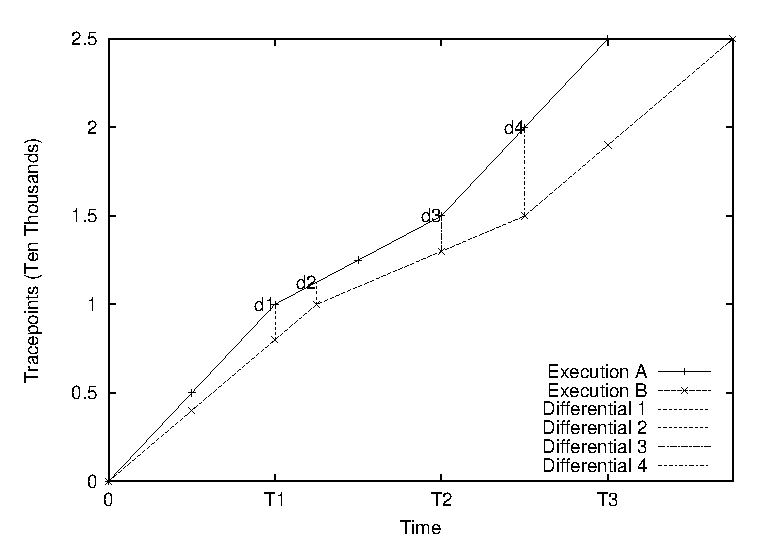
\includegraphics[width=0.9\columnwidth]{figures/executions_example.eps}
\caption{Executions Example}
\label{figure:executionsexample}
\end{figure}

A naive idea for exposing outliers is generating two clusterings using a one-degree Kmeans Clustering algorithm with all processes' number of tracepoints, and if the normalized variation of the two clusterings' means is larger than a threshold $T$, the clustering of processes with a mean value of $N$ less than the other one will be judged as outliers.

But the number of tracepoints is increased unevenly. We have proposed this dilemma at the instrumentation section. Four difference of two processes' number of tracepoints has been marked as $d_1, d_2, d_3, d_4$ at four different time point. Although process B is always 0.8X slower than process A, the difference of process A and process B is not increased along the whole timeline. An obvious case is $d_1 > d_2$, this may lead to the naive kmeans clustering approach missed process B when clustering outliers. Another type of mistake is some conditions just as $d_3 < d_4$, process B may just a little slower than process A, but judged as an outlier in the kmeans clustering naive approach. So there is no fixed threshold $T$ is appropriate for judging the outliers with the naive kmeans clustering approach.

To eliminate the mistake caused by false positive and false negative, An improved approach has been come up with. We proposed a new dynamic threshold $T_d$, which is determined by the threshold $T$, the mean of the increment of tracepoints of all processes $I_m$ and the increment of tracepoints of $i$th process $I_i$.

$$T_d = T \cdot (I_m / I_i)$$

As one of the assumptions is outliers is minority, the mean of the increment of tracepoints of all processes $I_m$ is near to the majority. When the variance of the means of clusterings decreased exceptionally like the case $d_1 > d_2$, the dynamic threshold $T_d$ decreased correspondingly, when the variance of the means of clusterings increased exceptionally like the case $d_3 < d_4$, the corresponding increase of $T_d$ comes after. So dynamic threshold $T_d$ can adaptive to the uneven increase of number of tracepoints perfectly. With this improvement approach for outliers clustering, NO2 can find out most of outliers but introducing little false positive. 